\documentclass[border=10pt]{standalone}

\usepackage{tikz}
\usepackage{tikzsymbols}
\usetikzlibrary{calc,patterns,shapes.geometric}

\def\centerarc[#1](#2)(#3:#4:#5){\draw[#1] ($(#2)+({#5*cos(#3)},{#5*sin(#3)})$) arc (#3:#4:#5);}

\begin{document}
	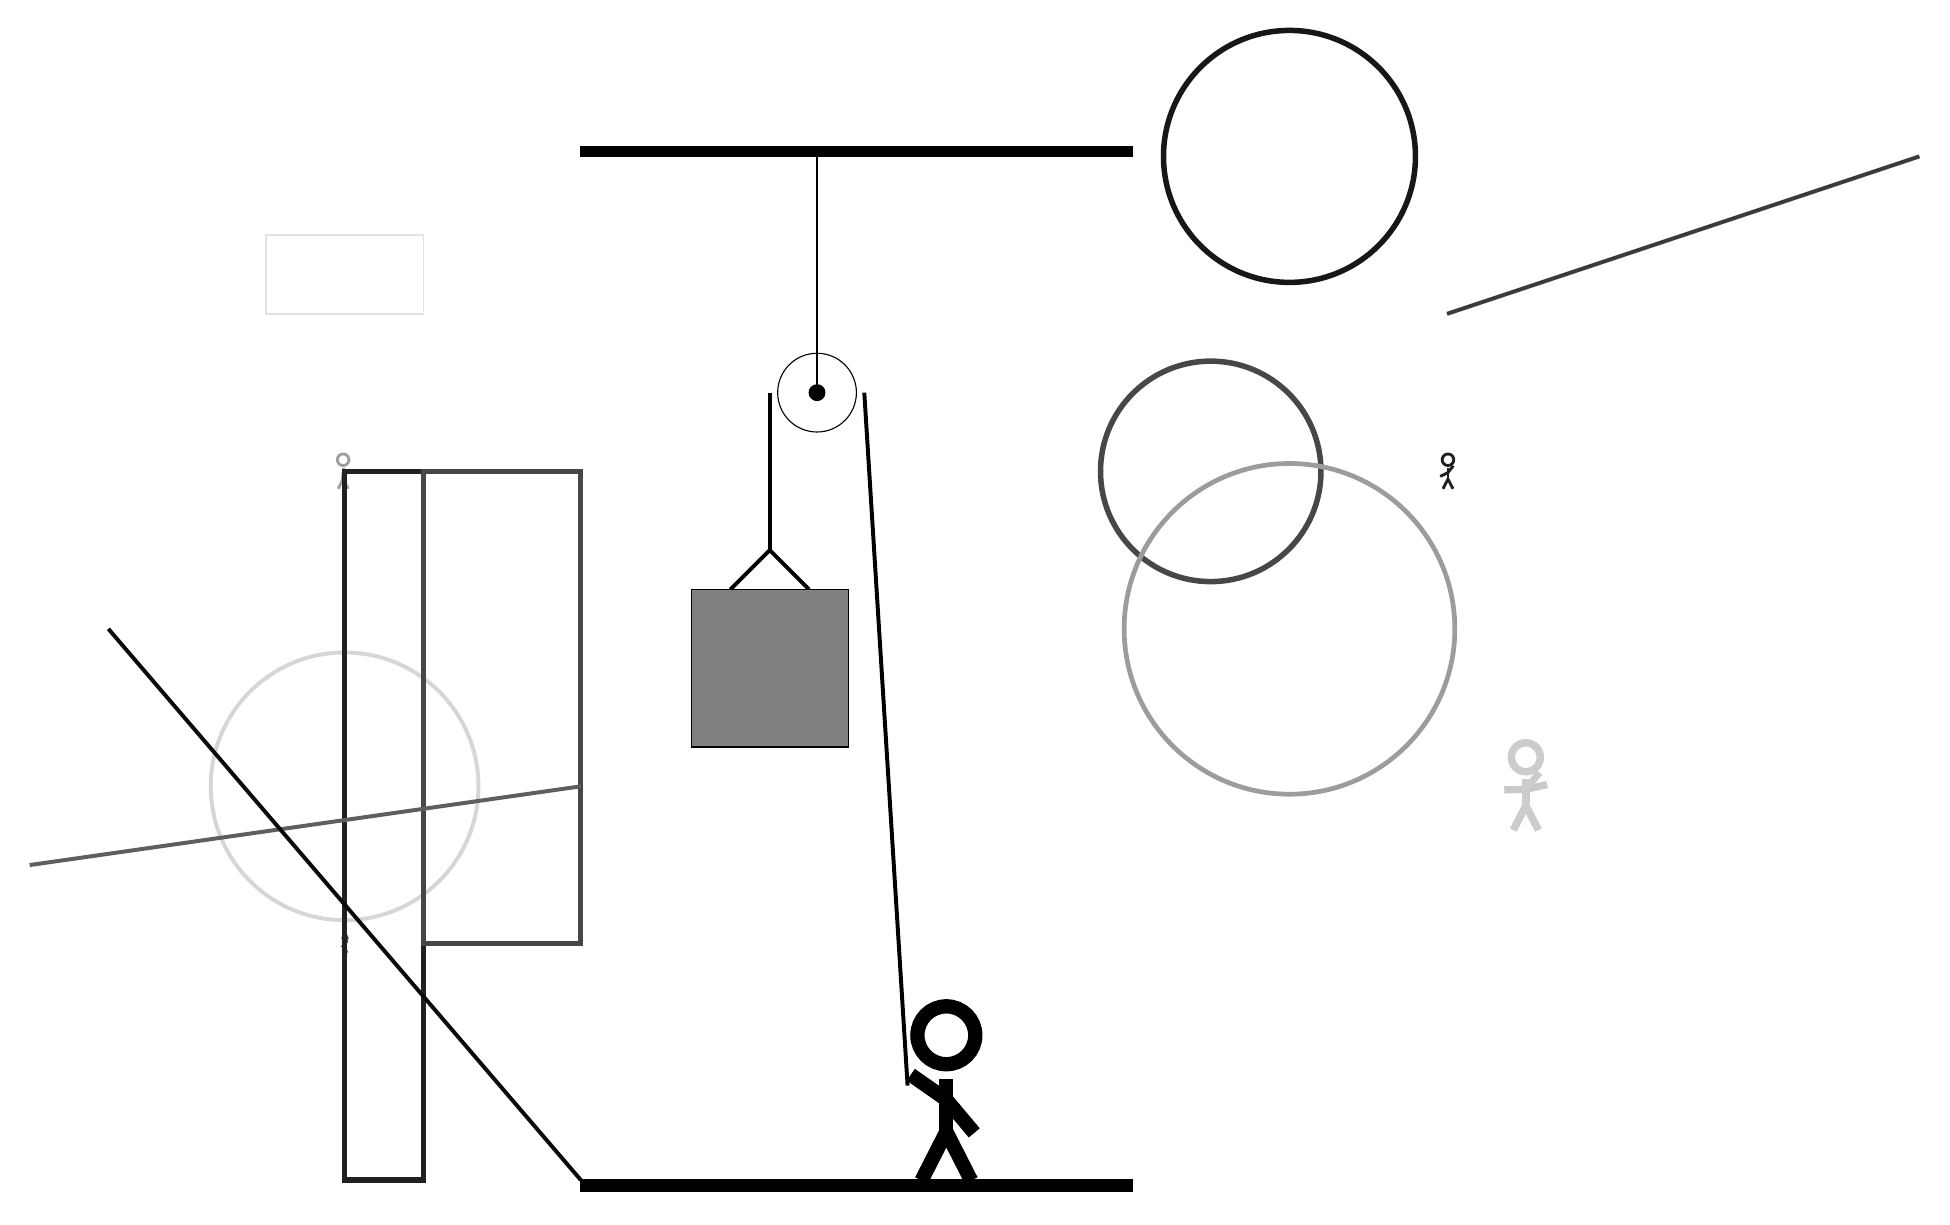
\begin{tikzpicture}
		%%%%% START %%%%%
		
		\draw[fill=black] (-2, 10) rectangle (5, 10.125);
		
		\draw (1, 7) circle (0.5);
		\draw[fill=black] (1, 7) circle (0.1);
		\draw (1, 10) -- (1, 7);
		
		\draw[line width=0.5mm] (-0.1, 4.5) -- (0.4, 5.0) -- (0.9, 4.5);
		\draw[fill=black!50] (-0.6, 4.5) rectangle (1.4, 2.5);
		
		\draw[line width=0.5mm] (0.4, 7) -- (0.4, 5.0);
		\centerarc[line width=0.5mm](1, 7)(0:180:0.6);
		\draw[line width=0.5mm](1.6, 7) -- (2.15, -1.8);
		
		\node at (2.6, -1.9) {\Strichmaxerl[10][-35][-50]};
		
		\draw [line width=0.7mm, color=black!72](6, 6) circle (1.4);
		
		\draw[line width=0.2mm, color=black!11] (-4, 9) rectangle (-6, 8);
		\node[line width=0.6mm, color=black!21] at (10, 2) {\Strichmaxerl[5][1][13]};
		\draw [line width=0.5mm, color=black!16](-5, 2) circle (1.7);
		\draw [line width=0.6mm, color=black!39](7, 4) circle (2.1);
		
		\node[line width=0.7mm, color=black!38] at (-5, 6) {\Strichmaxerl[2][83][0]};
		\node[line width=0.6mm, color=black!88] at (9, 6) {\Strichmaxerl[2][26][52]};
		
		\draw [line width=0.7mm, color=black!91](7, 10) circle (1.6);
		\node[line width=0.2mm, color=black!74] at (-5, 0) {\Strichmaxerl[1][30][50]};
		\node[line width=0.5mm, color=black!20] at (10, 2) {\Strichmaxerl[5][90][51]};
		\draw [line width=0.7mm, color=black!84](10, -1) circle (0.0);
		\draw[line width=0.3mm, color=black!15] (-2, 0) rectangle (-2, 4);
		\draw[line width=0.7mm, color=black!87] (-4, 6) rectangle (-5, -3);
		
		\draw[line width=0.5mm, color=black!77](9, 8) -- (15, 10);
		\draw[line width=0.6mm, color=black!72] (-4, 6) rectangle (-2, 0);
		\draw[line width=0.5mm, color=black!63](-2, 2) -- (-9, 1);
		\draw[line width=0.5mm, color=black!96](-2, -3) -- (-8, 4);
		
		\draw[fill=black] (-2, -3) rectangle (5, -3.15);
		
		%%%%% END %%%%%
	\end{tikzpicture}
\end{document}